\documentclass[letterpaper]{article}

% --- Packages
\usepackage[utf8]{inputenc}
\usepackage[T1]{fontenc}
\usepackage[margin=0.25cm]{geometry}
\usepackage{enumitem}
\usepackage{pdfpages}
\usepackage{multicol}
\usepackage{amsmath}
\usepackage{amssymb}
\usepackage[skip=1pt plus1pt, indent=0pt]{parskip}
\usepackage{enumitem}
\usepackage{graphicx}

% --- Data
\title{Introduction to electric circuits}
\author{Enrique Calderon}
\date{April 2024}

% --- Graphics path
\graphicspath{ {./img/} }

% --- Custom commands
\makeatletter
\let\thetitle\@title
\let\theauthor\@author
\makeatother
\newcommand{\compconj}[1]{%
    \overline{#1}%
}
\newcommand{\divline}{\noindent\makebox[\linewidth]{\rule{\textwidth}{0.4pt}}}
\newcommand{\taninv}{\tan^{-1}}
 
% Example of image adding
%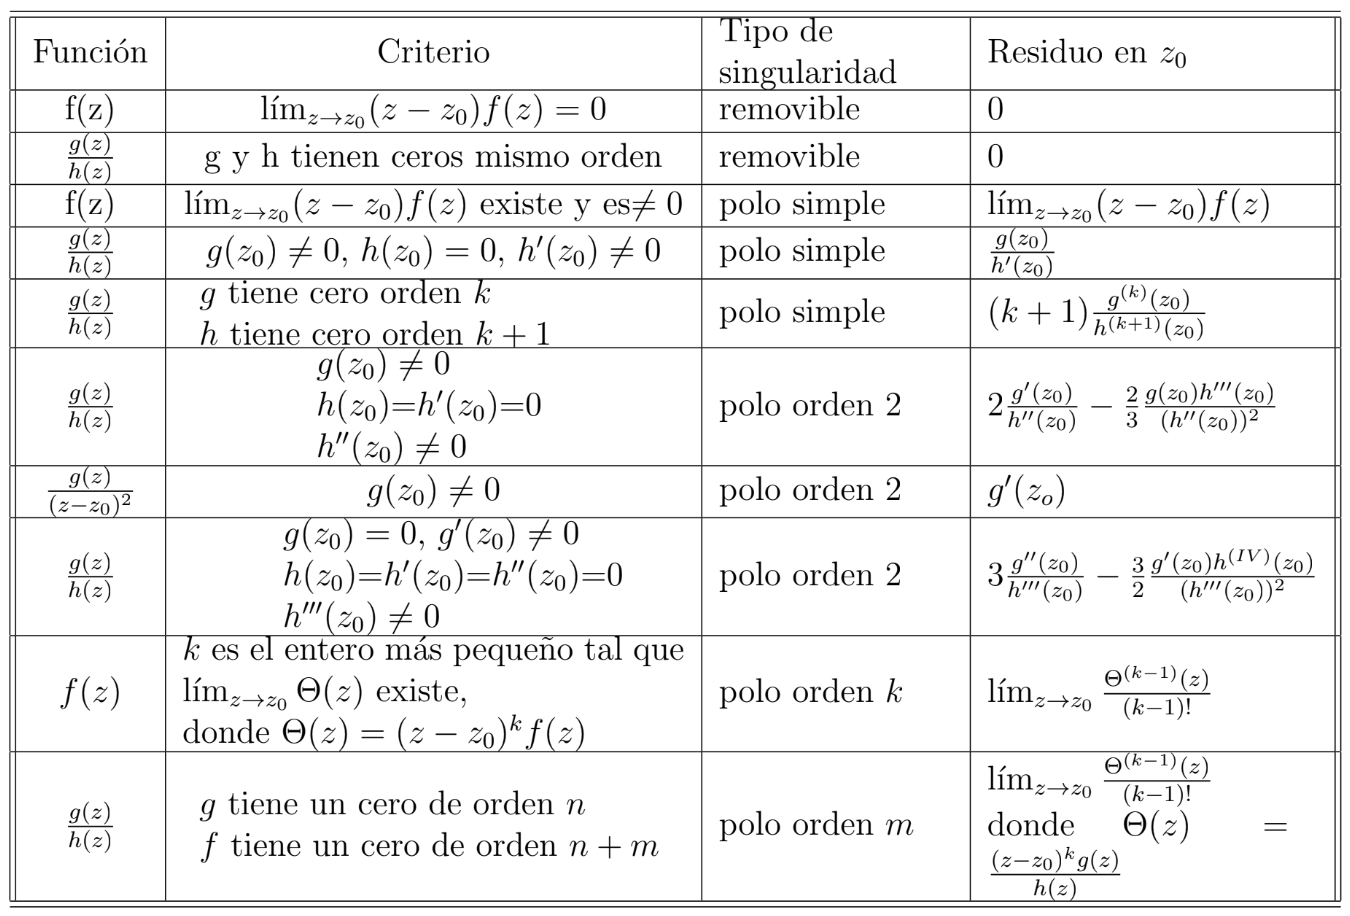
\includegraphics[width=0.8\textwidth]{ResidueTable}

% Remember to add divline between sections

\begin{document}
    \maketitle
    \divline
    
    \begin{multicols}{2}
        \section{Concepts and definitions}
        
        Electric current

        \[I = \frac{\delta Q}{\delta t} [A]\]

        Ampere unit

        \[1 [A] = \frac{1[C]}{1[S]}\]

        Number of free charge carriers

        \[n = \frac{\# e^{-}}{\mathbb{V}} \left[ \frac{1}{m^{3}} \right]\]

        Average speed of free charge carriers

        \[v_{p} = \frac{I}{n \left| q_{e} \right| A } \left[ \frac{m}{s} \right] \]

        Electric current density

        \[J = \frac{I}{A} \left[ \frac{A}{m^{2}} \right] = n q_{e} v_{p} \left[ \frac{A}{m^{2}} \right] \]

        Electric current density in a vector form

        \[\overline{J} = n q_{e} \overline{v}_{p} \left[ \frac{A}{m^{2}} \right] \]
    \end{multicols}
    \divline

    \begin{multicols}{2}
        \section{Ohm law}

        In vector form

        \[\overline{J} = \sigma \overline{E} \left[ \frac{A}{m^{2}} \right] = \frac{\overline{E}}{\rho} \left[ \frac{A}{m^{2}} \right] \] 

        Resistivity

        \[\rho = \frac{1}{\sigma} \left[ \Omega \cdot m \right] \]

        Resistivity according to temperature

        \[\rho = \rho_{0} \left[ 1 + \alpha (T - T_{0}) \right] \left[ \Omega \cdot m \right] \]

        Where:

        \begin{itemize}
            \item \(\rho\) : Resistivity of the material at a temperature \(T\).
            \item \(\rho_{0}\) : Resistivity of the material at \(20  \left[ ^\circ C \right] \)
            \item \(\alpha\) : Temperature coefficient of the material \(\left[ ^\circ C \right]^{-1} \)
        \end{itemize}

        Electric resistance

        \[R = \rho \frac{l}{A} \left[\Omega\right]\]

        Ohm unit

        \[1 \left[\Omega\right] = \frac{1[V]}{1[A]}\]

        Potential difference

        \[V_{ab} = R I \left[ V\right] \]

        Resistors colors

        \begin{center}
            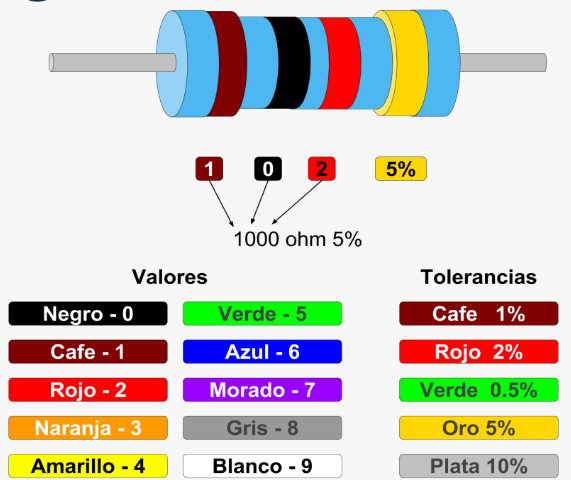
\includegraphics[width=0.25\textwidth]{ElectricidadyMagnetismo/img/resistance_colors.png}
        \end{center}
    \end{multicols}
    \divline

    \begin{multicols}{2}
        \section{Joule law}

        Electric power

        \[P = ( V_{ab} \cdot I ) [w]\]

        Watt unit

        \[1[w] = \frac{1[J]}{1[s]}\]

        Joule law

        \[P = R \cdot I^{2} = \frac{V^{2}}{R} [w]\]

        Dissipated energy

        \begin{align*}
            U_{R} & = P t & [J] \\
                & = V I t & [J] \\
                & = R I^{2} t & [J] \\
                & = \frac{V^{2}}{R} t & [J]
        \end{align*}
    \end{multicols}
    \divline

    \begin{multicols}{2}
        \section{Resistance connections}

        In series

        \[I = I_1 = I_2 = I_3 = ...\]
        \[V_{ad} = V_1 + V_2 + ... \]
        \[R_{eq} = \sum_{i = 1}^{n} R_i [\Omega] \]

        In parallel

        \[V_{ab} = V_1 = V_2 = V_3 = ...\]
        \[I = I_1 + I_2 + I_3 + ...\]
        \[R_{eq} = \left( \sum_{i=1}^{n} \frac{1}{R_{i}} \right)^{-1} [\Omega]\]
    \end{multicols}
    \divline

    \begin{multicols}{2}
        \section{Electromotive Force}

        It is defined as

        \[\varepsilon = \frac{w}{q} = \int \overline{E} \cdot d \overline{l} [V]\]

        Ideal electromotive force

        \begin{align*}
            P_{\text{ideal}} & = \varepsilon I & [w] \\
            U_{\text{ideal}} & = P t & [J] \\
            U_{\text{ideal}} & = \varepsilon I t & [J]
        \end{align*}

        Real electromotive force

        \begin{align*}
            P_{\text{real}} & = P_{\text{ideal}} - P_{ri} & [w] \\
            P_{\text{real}} & = \varepsilon I - r_{i} I^{2} & [w] \\
            U_{\text{real}} & = P_{\text{real}} t & [J] \\
            U_{\text{real}} & = ( \varepsilon I - r_{i} I^{2} ) t & [J]
        \end{align*}
    \end{multicols}
    \divline

    \begin{multicols}{2}
        \section{Nomenclature}

        \begin{itemize}
            \item Branch: A a electric device with two terminals.
            \begin{center}
                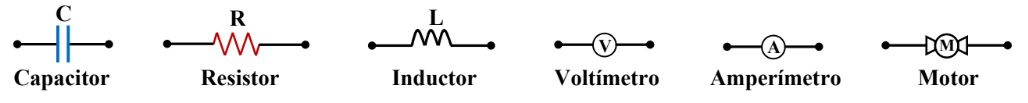
\includegraphics[width=0.45\textwidth]{ElectricidadyMagnetismo/img/nomenclature.png}
            \end{center}
            \item Principal branch: The branch or branches that connect two adjacent principal nodes.
            \item Node: Union of two or more branches.
            \item Principal node: Union of three or more branches.
            \item Mesh: Branch set connected in a closed trajectory.
        \end{itemize}
    \end{multicols}
    \divline

    \begin{multicols}{2}
        \section{Kirchhoff Laws}

        \begin{itemize}
            \item LCK: The sum of electric current in a node is equal to 0. \(\sum_{k=1}^{n} I_{k} = 0\). If the current enters is positive and if it exits is negative.
            \item Independent equations in  node (EIN):  Its equal to the number of principal nodes minus one. \(EIN = N_{p} - 1\)
            \item LVK: The sum of potential differences in a mesh with closed trajectory is zero. \(\sum_{k=1}^{n} V_{k} = 0\). \((- \implies +)\) is positive and \((+ \implies -)\) is negative.
            \item Independent equation in meshes (EIM): Its equal to the number of principal meshes minus the number of independent nodes. \(EIM = R_{p} - EIN\).
        \end{itemize}
    \end{multicols}
    \divline

    \begin{multicols}{2}
        \section{Introduction to RC circuits}

        Initial electric current, maximum electric current

        \[i_0 = \frac{E}{R}[A]\]

        Total electric current

        \[q_{\text{max}} = C \varepsilon [C]\]

        Getting the current according the time

        \[i(t) = \frac{\varepsilon}{R} e^{- \frac{t}{RC}} [A]\]

        Tau constant: \(\tau = RC [s]\)

        We can obtain time as:

        \[t = -RC \ln{\frac{i}{i_0}} [s]\]

        Determine electric charge on a capacitor

        \[q(t) = C \varepsilon ( 1 - e^{- \frac{t}{RC}} )[C]\]

        Determine potential difference on a capacitor

        \[V_c (t) = \varepsilon (1 - e^{- \frac{t}{RC}}) [V]\]

        Determine potential difference on a resistor

        \[V_R (t) = \varepsilon e^{- \frac{t}{RC}} [V]\]

        Determine electric charge on a capacitor when discharging

        \[q(t) = C \varepsilon e^{- \frac{t}{RC}} [C]\]

        Determine the electric current in the circuit

        \(i(t) = - \frac{\varepsilon}{R} e^{- \frac{t}{RC}} [A]\)
        
    \end{multicols}
    
\end{document}